\documentclass{beamer}
\usepackage{beamerthemeshadow}
\usepackage[english]{babel}

\begin{document}
\title{Modeling Variable Throughput Channels with Stochastic ODEs}  
\author{D. Masi, P. Pegus II , J. M. Wong}
\date{\today} 

\frame{\titlepage} 

\frame{\frametitle{Outline}\tableofcontents} 

\section{Introduction} {
	\frame{\frametitle{Introduction} {
		\begin{figure}[H]
		\centering
		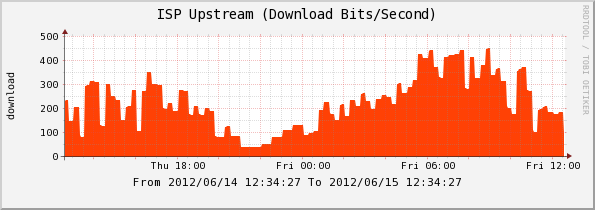
\includegraphics[scale=.40]{Images/throughput.png}
		\end{figure}
		Stochastic differential equations are often used to model the nondeterministic behavior of network channels in computer science.
		}
	}
	\subsection{Networking Basics} {
		\frame{\frametitle{Networking Basics} {
			A \textbf{Channel} is the medium through which a message propagates from sender to receiver.
			\begin{figure}[H]
			\centering
			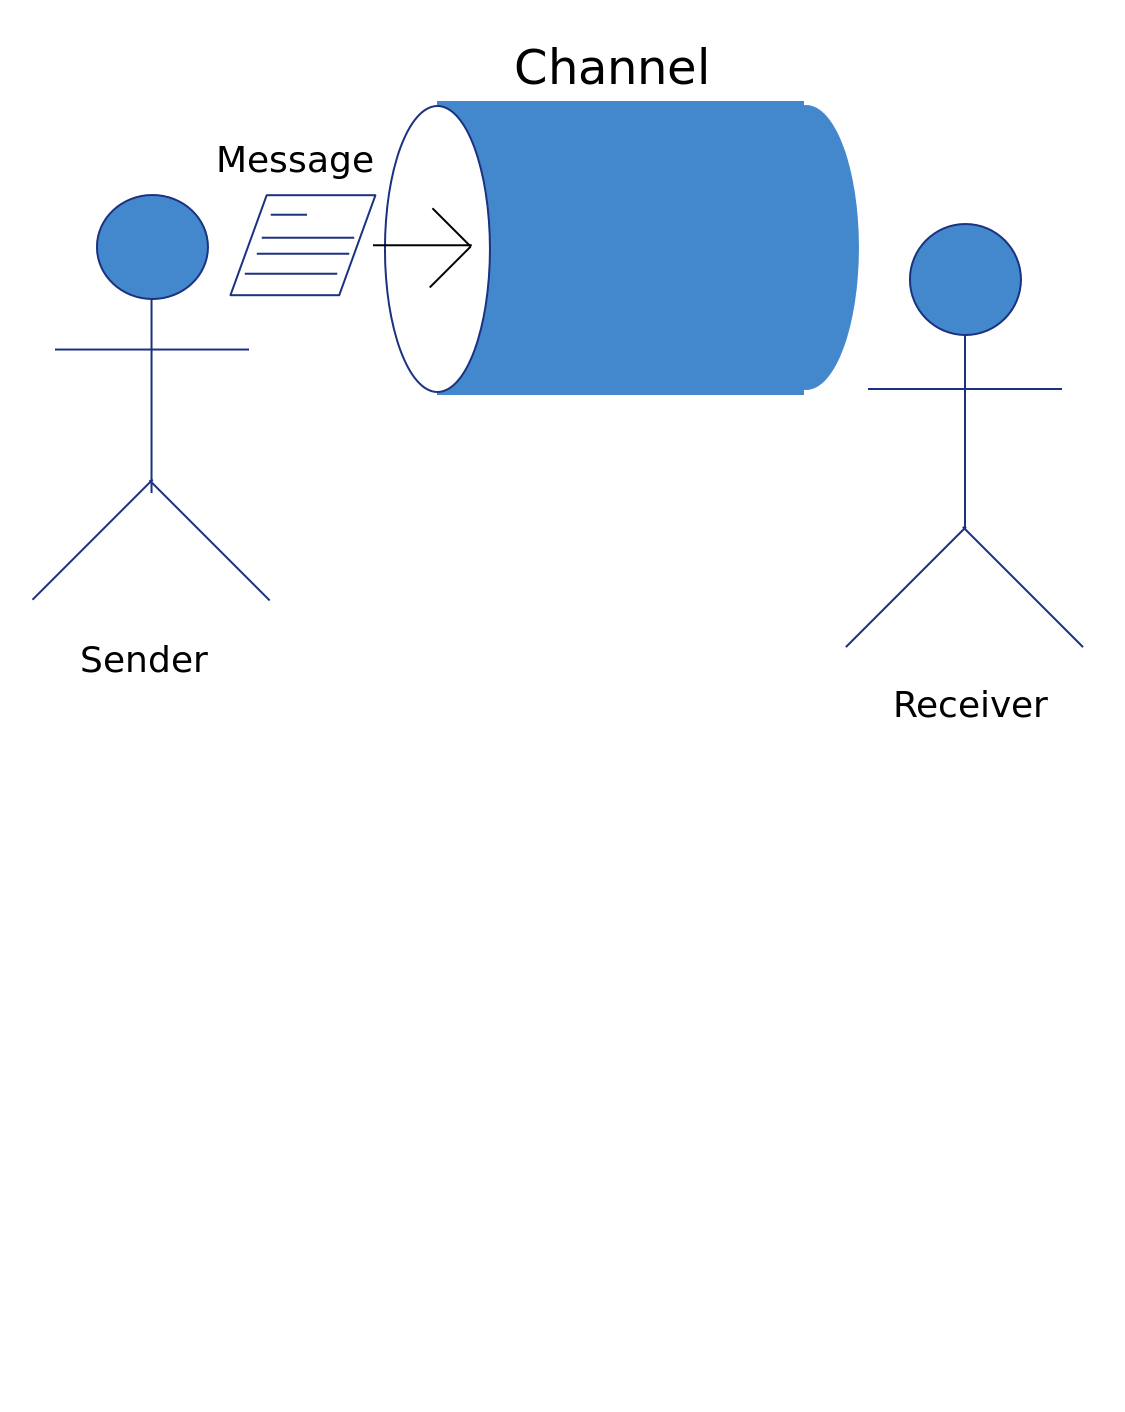
\includegraphics[scale=.20]{Images/network_components.png}
			\end{figure}
			}
		}
	}
	\subsection{Channel Characteristics} {
		\frame{\frametitle{Channel Characteristics} {
			\begin{figure}[H]
			\centering
			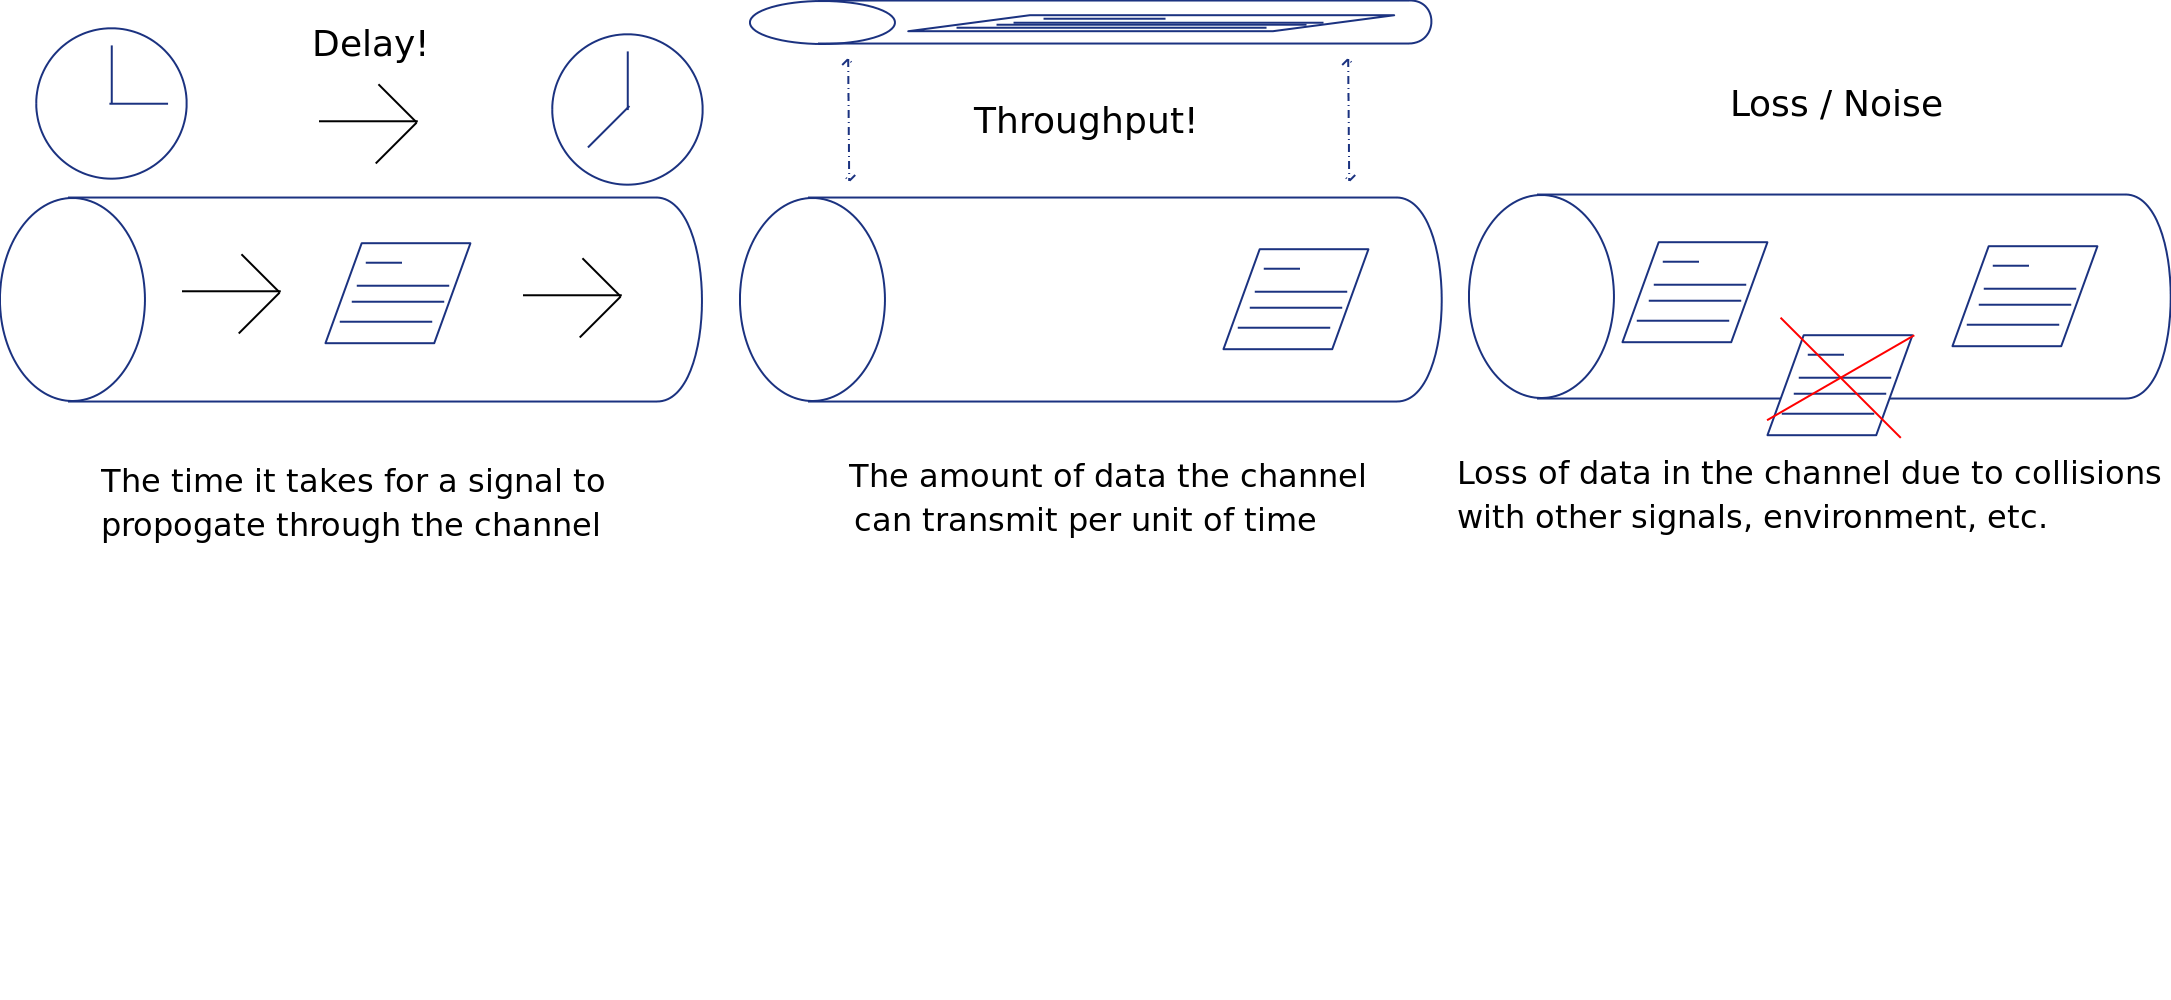
\includegraphics[scale=.15]{Images/channel_characteristics.png}
			\end{figure}
			}
		}
	}
	\subsection{Throughput} {
		\frame{\frametitle{Throughput} {
			We model the variations in throughput with a simple algorithm that combines deterministic and probabilistic influences.
			\begin{description}
				\item[Deterministic] \hfill \\
					- \textbf{Constant}: The obvious case of constant throughput. \\
					- \textbf{Periodic}: The throughput a wireless device achieves can vary periodically as it changes location. \\
					- \textbf{Burst}: Internet Service Providers may give high initial throughput rates. \\
				\item[Probabilistic] \hfill \\
					- \textbf{Periodic}: Can model the chance of loss. \\
					- \textbf{Approaching zero}: When communication within a channel begins, there may be greater risk of message collisions. \\
			\end{description}
			}
		}
	}
	\subsection{Application} {
		\frame{\frametitle{Application} {
			Modeling a variable throughput channel is good, but we'd really like to test an application using it as a communication medium. So we simulate
			an adaptive quality video streaming application which uses algorithms that try to maximize video frame quality while still having each frame
			arrive to the receiver on time.
				\begin{figure}[H]
				\centering
				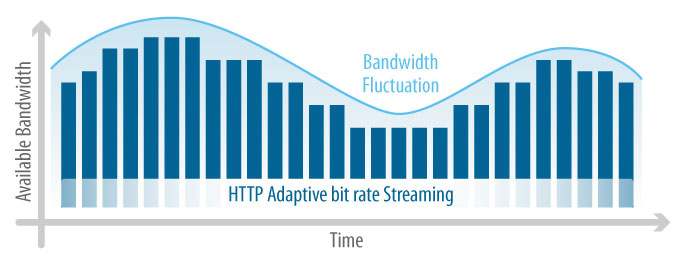
\includegraphics[scale=.45]{Images/adaptive_streaming.jpg}
				\end{figure}
			}
		}
	}
	\subsection{Experiment Framework} {
		\frame{\frametitle{Experiment Framework} {
			\begin{description}
				\item[Inputs] \hfill \\
					- \textbf{Initial Channel Throughput} \\
					- \textbf{Deterministic Change in Throughput} \\
					- \textbf{Stochastic Change in Throughput} \\
					- \textbf{Adaptive Streaming Algorithm} \\
					- \textbf{Video} \\
					- \textbf{Video Compression Algorithm} \\
				\item[Outputs] \hfill \\
					- \textbf{Realized Channel Throughput}: can be used to rerun experiment with different algorithms on the same channel rate \\
					- \textbf{Frame Quality}: can be used to compare video quality achieved with different algorithms \\
			\end{description}
			}
		}
	}
}

\section{Image Compression} {
	\frame{\frametitle{Image Compression} {
		\begin{figure}[H]
		\centering
		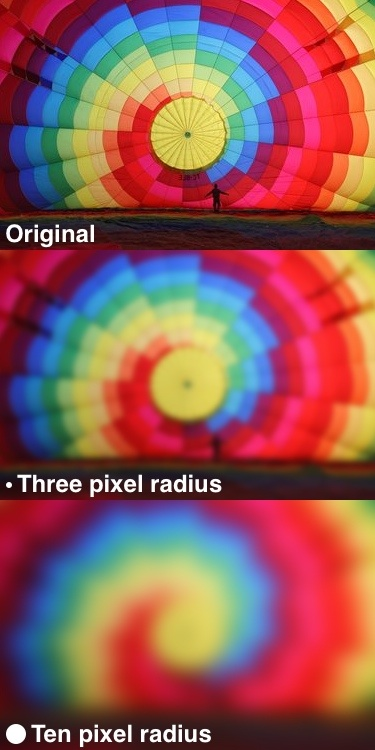
\includegraphics[scale=.25]{Images/Gaussian_blur_example.png}
		\end{figure}
		}
	}
	\subsection{Compression Using Low Pass} {
		\frame{\frametitle{Compression Using Low Pass} {
		\begin{figure}[H]
		\centering
		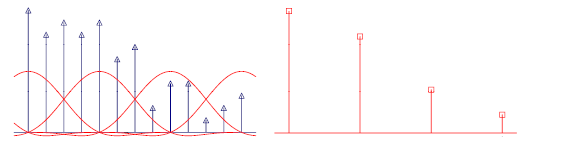
\includegraphics[scale=.67]{Images/LowPassFiltering.png}
		\end{figure}
			}
		}
	}
	\subsection{Compression Using Average} {
		\frame{\frametitle{Compression Using Average} {
		\begin{figure}[H]
		\centering
		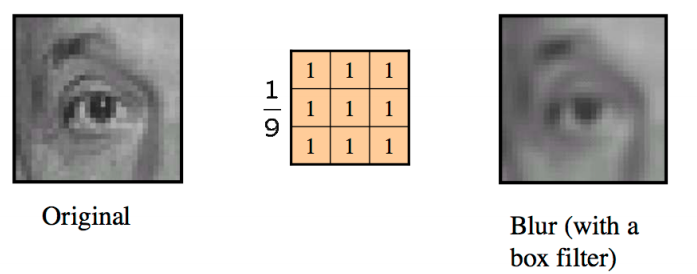
\includegraphics[scale=.40]{Images/BlurBoxFilter.png}
		\end{figure}
			}
		}
	}
	\subsection{Sharpening} {
		\frame{\frametitle{Sharpening} {
		\begin{figure}[H]
		\centering
		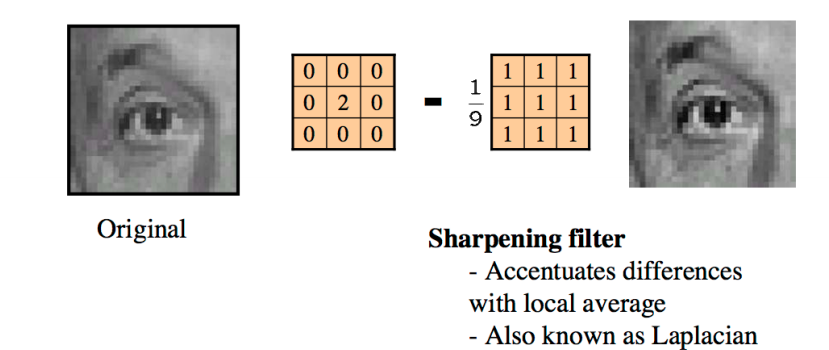
\includegraphics[scale=.30]{Images/Sharpening1.png}\\
		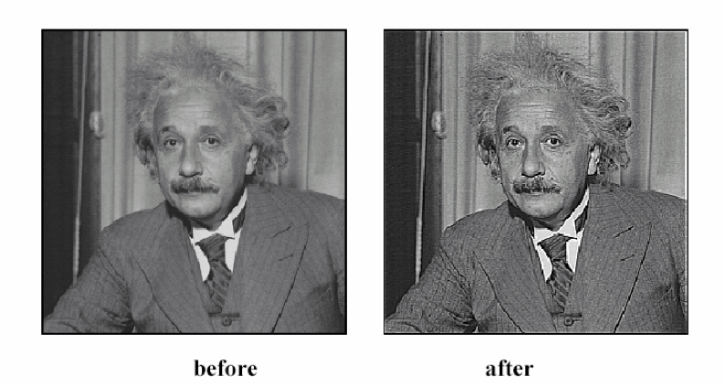
\includegraphics[scale=.30]{Images/Sharpening2.png}
		\end{figure}
			}
		}
	}
}

\section{Implementation}{
\subsection{Euler-Marauyama Method} {
		\frame{\frametitle{Euler-Marauyama Method} {
			We approximate the solution by assigning y-values $w_0 < w_1 < w_2 < \cdots < w_n$ at discretized $t$, given the SDE IVP
			\begin{equation}
				dy(t) = f(y,t)dt+g(t,y)dB_t
			\end{equation}
			\begin{equation}
				y(a) = y_a
			\end{equation}
			\begin{figure}[H]
			\centering
			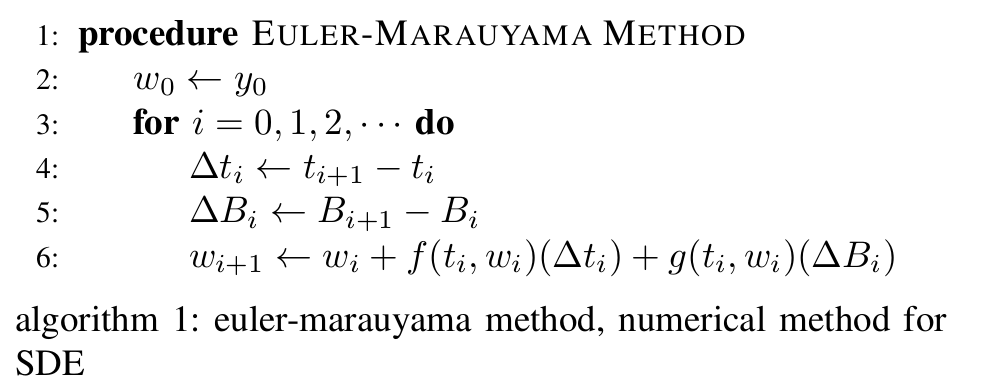
\includegraphics[scale=.3]{Images/euler.png}
			\end{figure}
			}
		}
	}


}
\section{Demonstration}{
	\frame{\frametitle{Demonstration} {
		\begin{figure}[H]
		\centering
		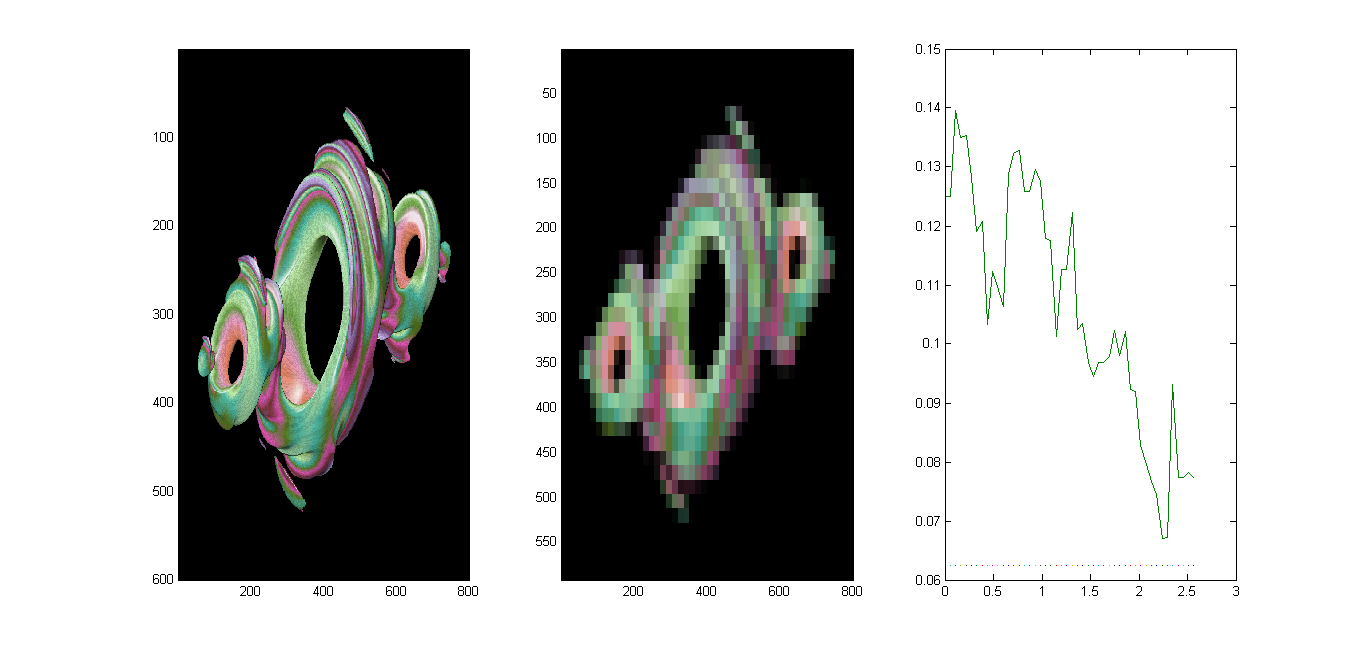
\includegraphics[scale=.30]{Images/img.png}
		\end{figure}
}

}

}

\end{document}
\section{Demonstration}{
	\frame{\frametitle{Demonstration} {
		\begin{figure}[H]
		\centering
		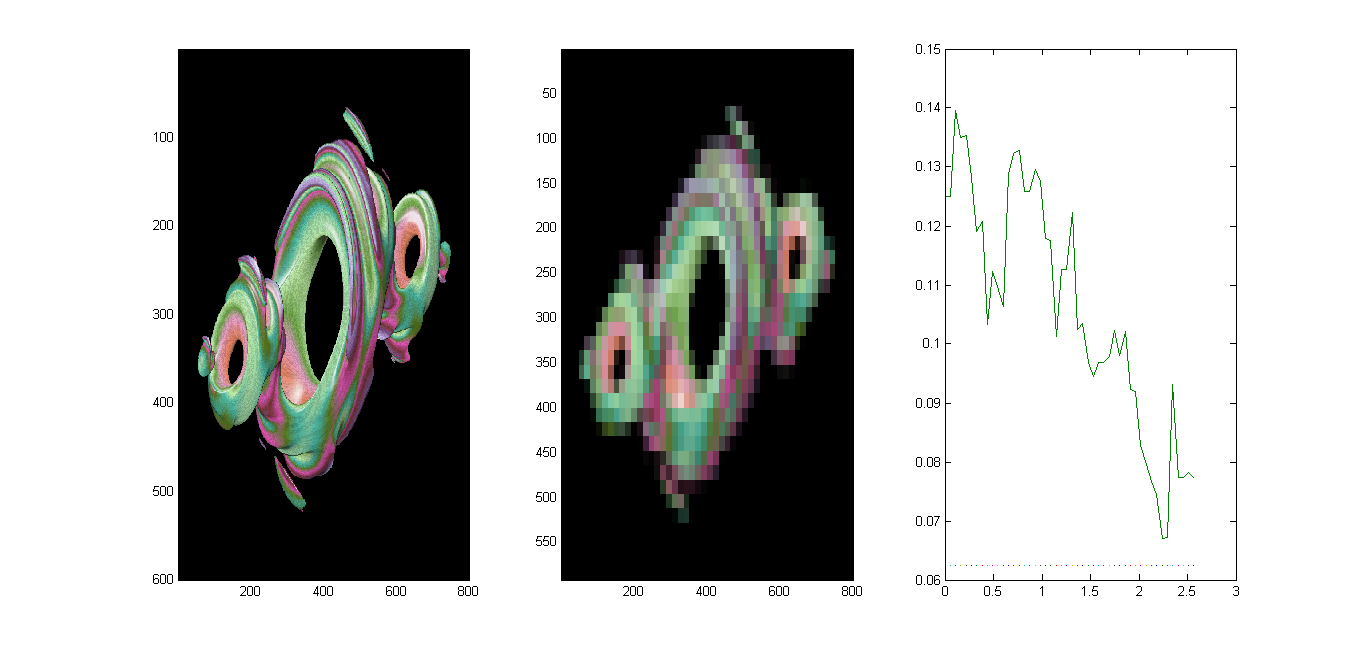
\includegraphics[scale=.30]{Images/img.png}
		\end{figure}
}

}

}

\end{document}

